% 图库结构说明及树状图
\documentclass[UTF8]{ctexart}
\usepackage{enumitem}
\usepackage{geometry}
\geometry{a4paper, margin=2cm}
\usepackage[edges]{forest}
\usepackage{xcolor}
\usepackage{verbatim}
\usepackage{graphicx}
\usepackage{float}

% ---- 颜色与图标定义 ---------------------------
\definecolor{foldercolor}{RGB}{124,166,198}

\tikzset{ pics/folder/.style={ code={ \node[inner sep=0pt, minimum size=#1](-foldericon){}; \node[folder style, inner sep=0pt, minimum width=0.3*#1, minimum height=0.6*#1, above right, xshift=0.05*#1] at (-foldericon.west){}; \node[folder style, inner sep=0pt, minimum size=#1] at (-foldericon.center){}; } }, pics/folder/.default={20pt}, folder style/.style={ draw=foldercolor!80!black, top color=foldercolor!40, bottom color=foldercolor } }

\forestset{ is file/.style={ edge path'/.expanded={ ([xshift=\forestregister{folder indent}]!u.parent anchor) |- (.child anchor) }, inner sep=1pt }, this folder size/.style={ edge path'/.expanded={ ([xshift=\forestregister{folder indent}]!u.parent anchor) |- (.child anchor) pic[solid]{folder=#1} }, inner ysep=0.6*#1 }, folder tree indent/.style={ before computing xy={l=#1} }, folder icons/.style={ folder, this folder size=#1, folder tree indent=3*#1 }, folder icons/.default={12pt}, }

% ------------------------------------------------
\begin{document}
	% -------- 图库目录说明 -------------------------
	\section*{图库目录说明}
	\begin{enumerate}
		\item \textbf{根目录:}\verb|图库|,为所有图片的总仓库。

		\item \textbf{第一层:大类文件夹}(如 \verb|BXG|、\verb|TH|、\verb|MT| 等),每个大类文件夹存放该类产品的全部图片。

		\item \textbf{第二层:风格文件夹}(如 \verb|风格1|、\verb|风格2| 等),用于区分同一大类下的不同视觉风格或系列。

		\item \textbf{第三层:SKU 文件夹}(如 \verb|BGX22|、\verb|ZX84| 等)。有时一个
			SKU 文件夹也可能包含多个相近的 SKU。

		\item \textbf{SKU 文件夹内容说明:}
			\begin{itemize}
				\item 主图、详情图、尺寸图等直接放在 SKU 文件夹下,常见命名如 \verb|1.jpg|、\verb|详情图1.jpg|、\verb|尺寸图.jpg|。
					\begin{itemize}
						\item 软件根据文件名判断图片类型。尺寸图文件名需包含“尺寸图”,详情图同理。主图文件名可自定义。
					\end{itemize}

				\item 所有“选项图”需统一放在 SKU 文件夹下的子文件夹 \verb|选项图| 中,内部可进一步细分:
					\begin{itemize}
						\item 文件名中禁止使用 \verb|*|,请使用下划线 \verb|_| 替代。

						\item \verb|带数量|:图片中包含包装数量(如
							\verb|BGX22-3_7mm.jpg|)。

						\item \verb|不带数量|:图片中不含包装数量(如
							\verb|BGX22-3_7mm.jpg|)。
					\end{itemize}
			\end{itemize}
	\end{enumerate}

	% -------- 树状图 -------------------------------
	\section*{图库结构树}
	\begin{forest}
		for tree={ font=\sffamily, grow'=0, folder indent=.9em, folder icons, edge=- }
		[图库 [$\enskip$ BXG, this folder size=12pt [$\enskip$风格1 [$\enskip$BGX22
		[尺寸图.jpg, is file] [详情图1.jpg, is file] [详情图2.jpg, is file] [1.jpg,
		is file] [2.jpg, is file] [...jpg, is file] [$\enskip$选项图 [$\enskip$带数量
		[{BGX22-3\^{}7mm.jpg}, is file] [{BGX22-4\^{}9mm.jpg}, is file] [FZ173.jpg, is
		file] ] [$\enskip$不带数量 [...jpg, is file] ] [(固定数量的选项图)] ] ] [$\enskip$BGX24]
		[$\enskip$BGX25] [$\enskip$BGX26] ] [$\enskip$风格2] [$\enskip$...] ] [$\enskip$HDS
		[$\enskip$风格1] ] [$\enskip$FZ] [$\enskip$ZX] ]
	\end{forest}

  % -------- 图片举例 -------------------------------
  \section*{插图示例}

  \begin{figure}[H]
    \centering
    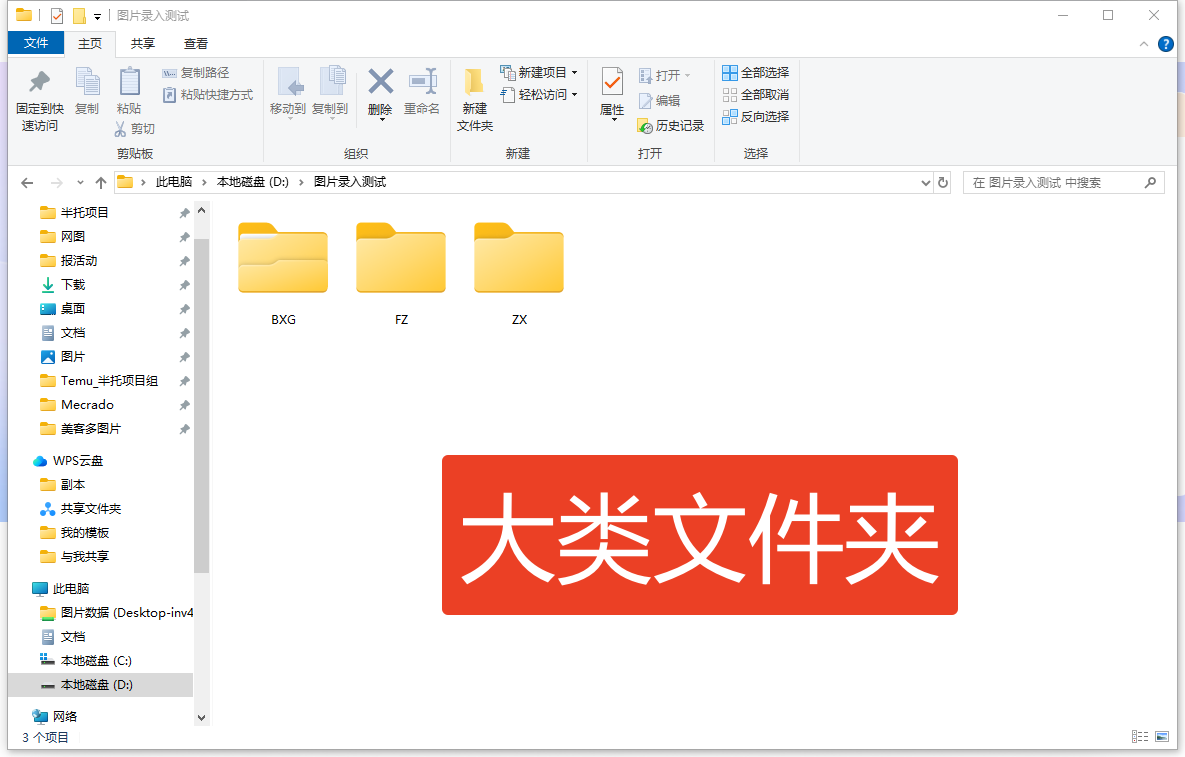
\includegraphics[width=0.6\textwidth]{image/image.png}
    \caption{大类文件夹}
  \end{figure}

  \begin{figure}[H]
    \centering
    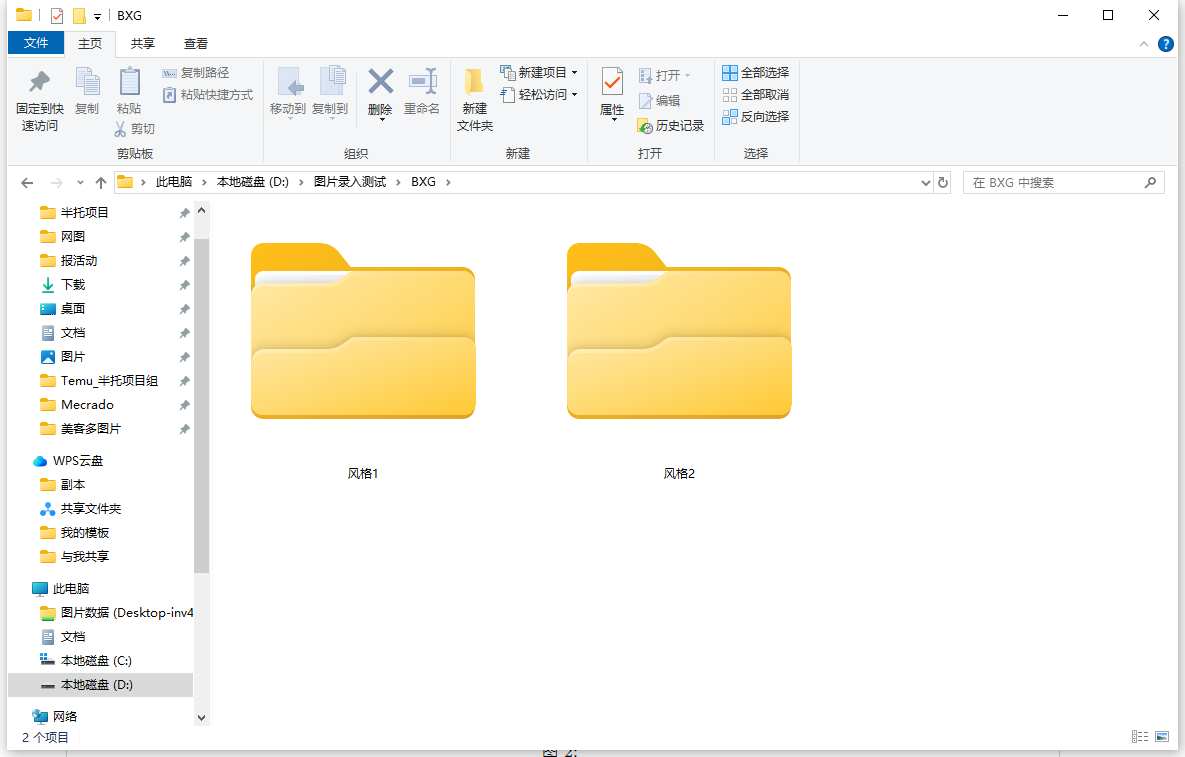
\includegraphics[width=0.6\textwidth]{image/image copy.png}
    \caption{风格文件夹}
  \end{figure}

  \begin{figure}[H]
    \centering
    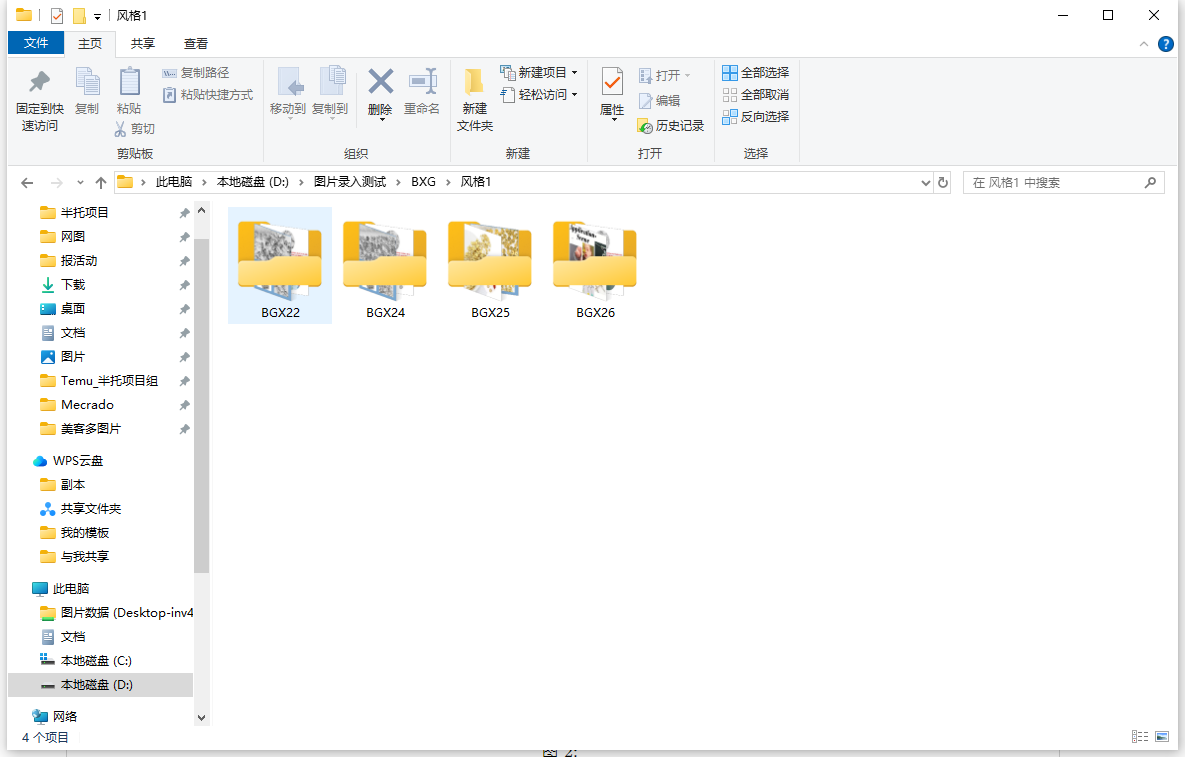
\includegraphics[width=0.6\textwidth]{image/image copy 2.png}
    \caption{sku文件夹}
  \end{figure}

  \begin{figure}[H]
    \centering
    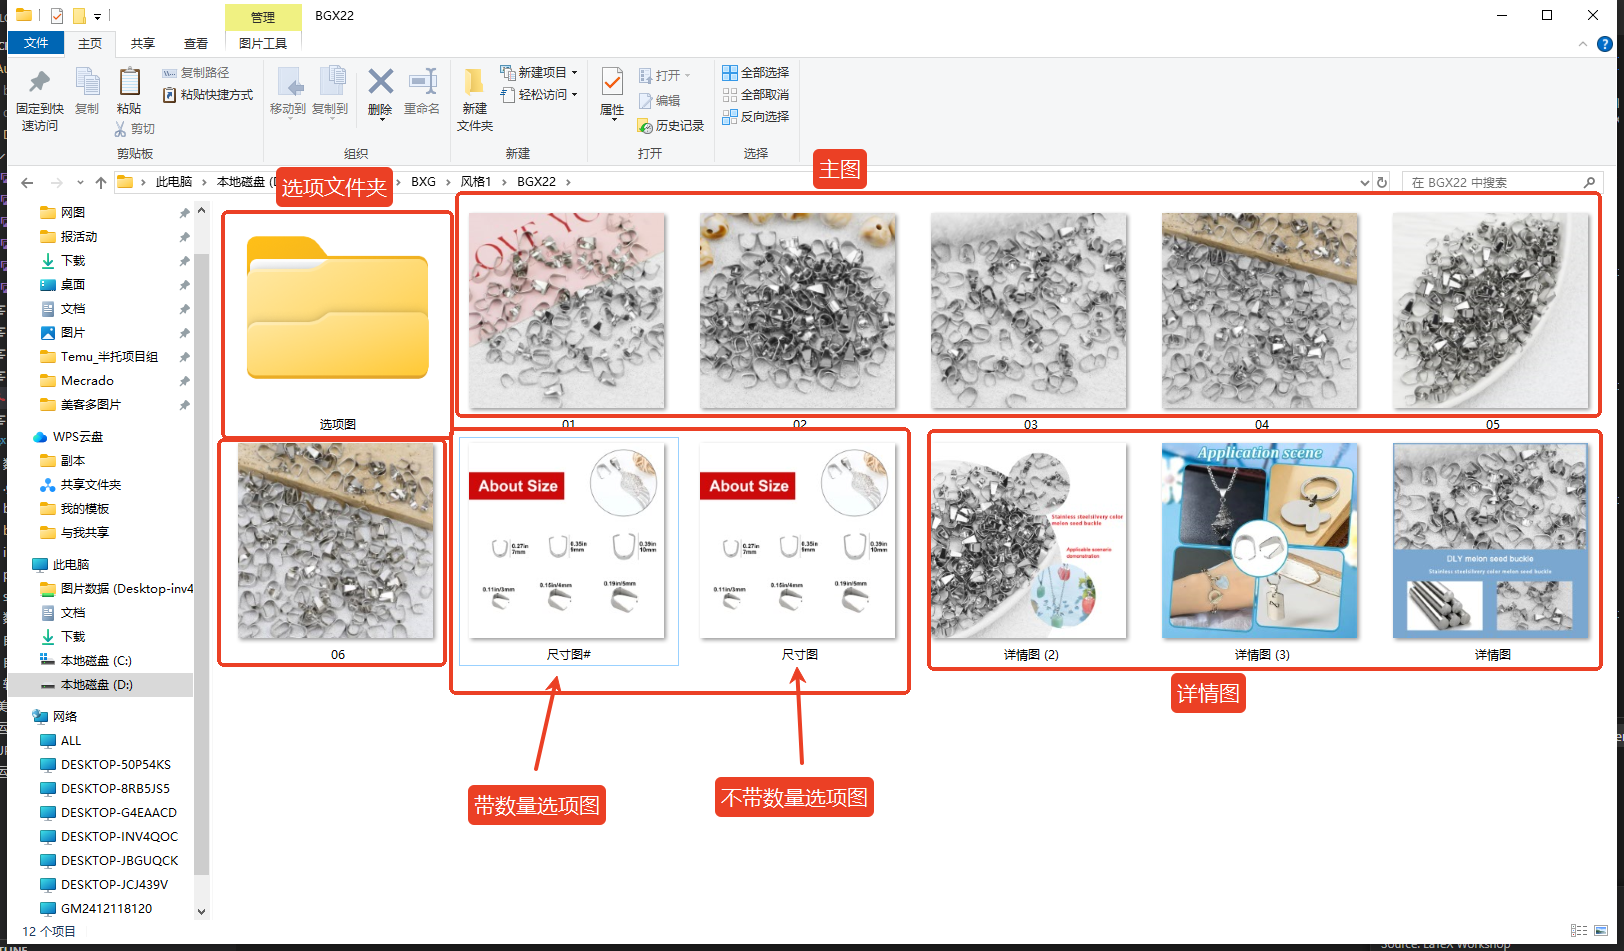
\includegraphics[width=0.6\textwidth]{image/image copy 6.png}
    \caption{图片文件夹}
  \end{figure}

  \begin{figure}[H]
    \centering
    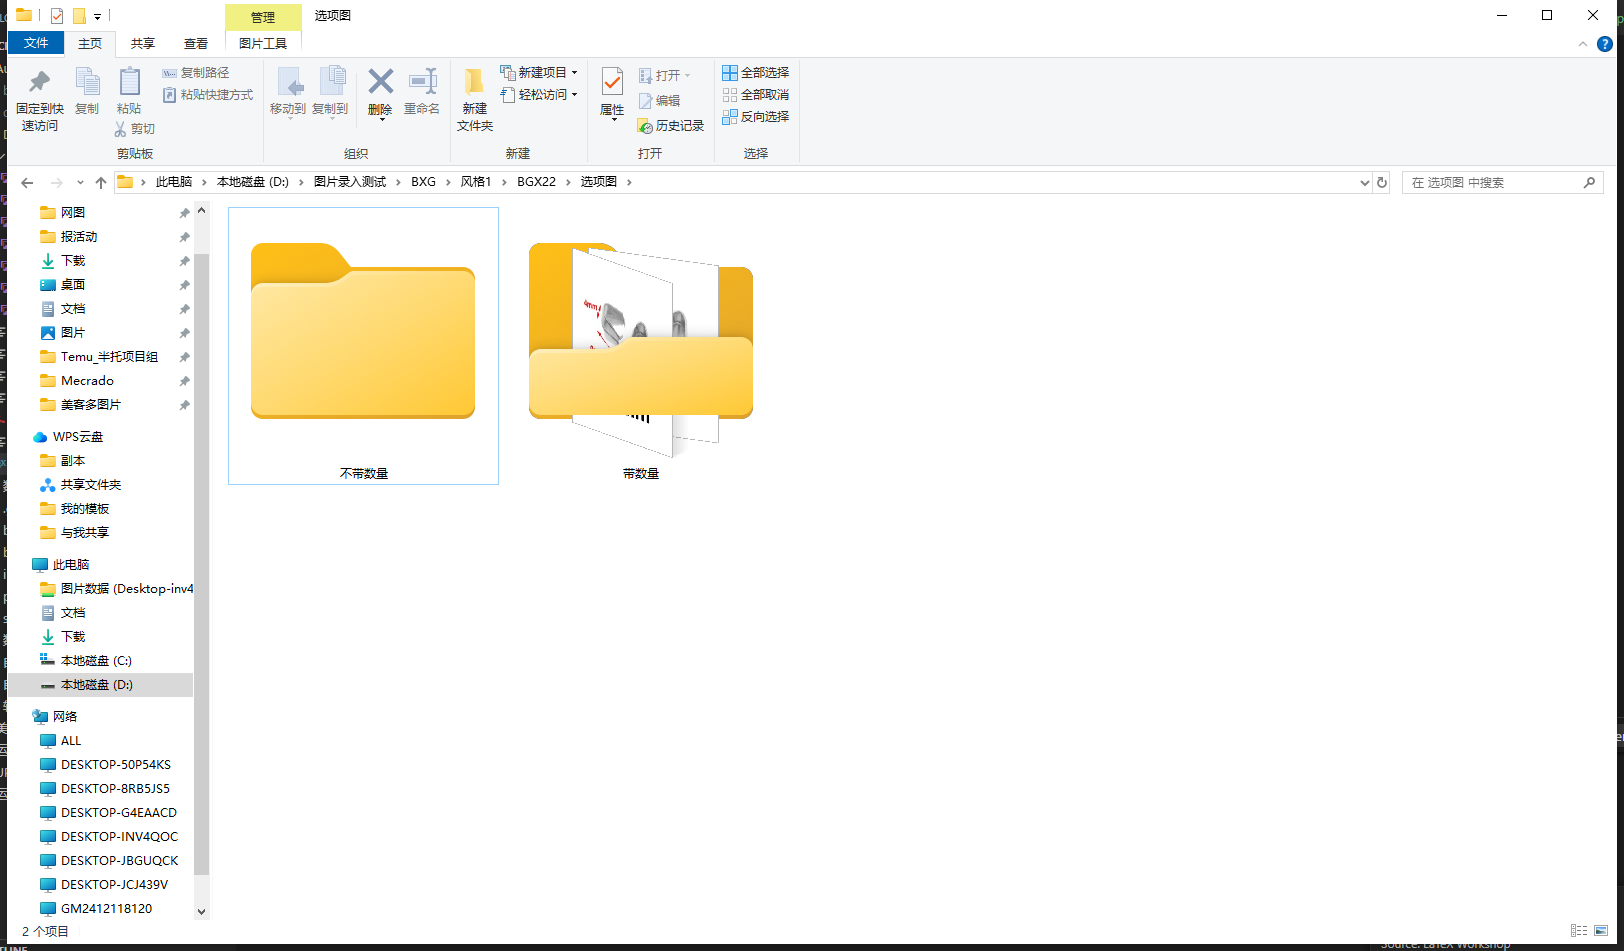
\includegraphics[width=0.6\textwidth]{image/image copy 7.png}
    \caption{选项图文件夹}
  \end{figure}

  \begin{figure}[H]
    \centering
    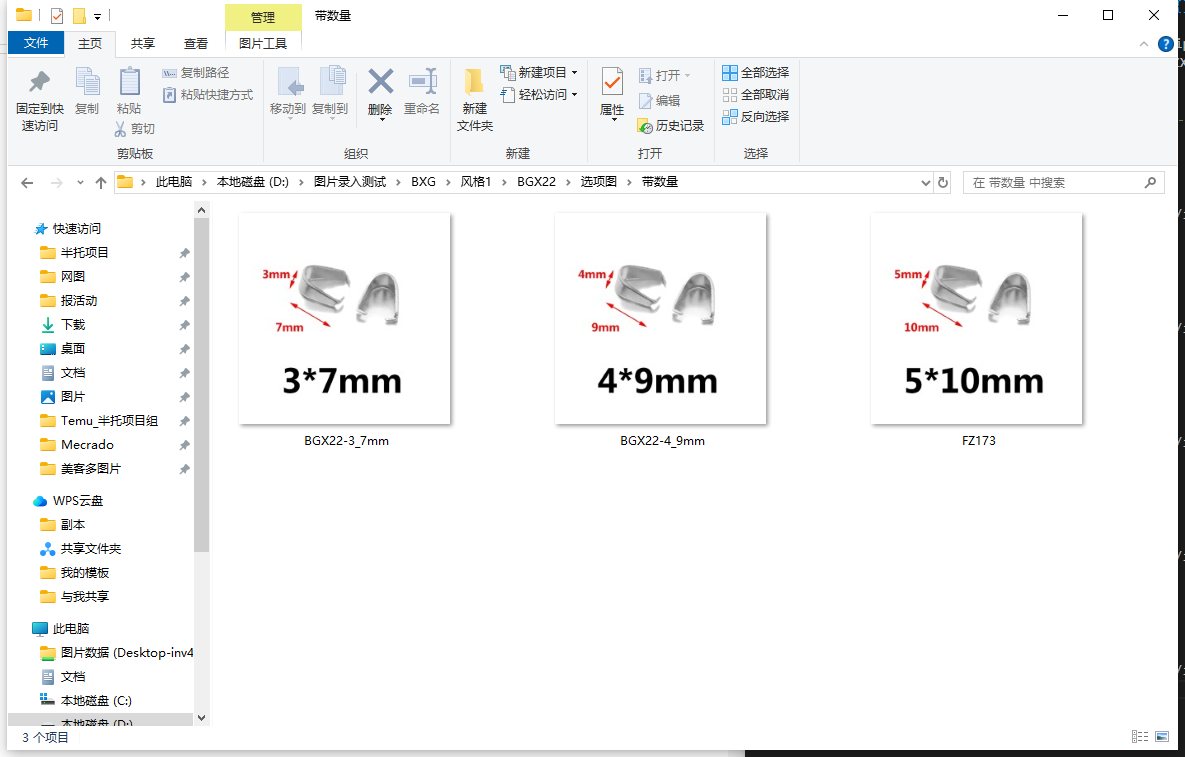
\includegraphics[width=0.6\textwidth]{image/image copy 5.png}
    \caption{带数量文件夹}
  \end{figure} 
\end{document}